\documentclass{report}
\usepackage[margin=1in, paperwidth=8.5in, paperheight=11in]{geometry}
%Math packages%
\usepackage{amsmath}
\usepackage{amsthm}
%Spacing%
\usepackage{setspace}
\onehalfspacing
%Lecture number%
\newcommand{\lectureNum}{3}
%Variables - Date and Course%
\newcommand{\curDate}{January 10, 2017}
\newcommand{\course}{CS 251}
\newcommand{\instructor}{Stephen Mann}
%Defining the example tag%
%\theoremstyle{definition}%
\newtheorem{ex}{Example}[section]
%Setting counter given the lecture number%
\setcounter{chapter}{\lectureNum{}}
%Package to insert code%
\usepackage{listings}
\usepackage{courier}
\usepackage{xcolor}
\lstset { %
    tabsize=2,
    breaklines=true,
    language=C++,
    backgroundcolor=\color{blue!8}, % set backgroundcolor
    basicstyle=\footnotesize\ttfamily,% basic font setting
}
%Package used to draw circuits%
\usepackage{circuitikz}
\begin{document}
%Note title%
\begin{center}
\begin{Large}
\textsc{\course{} | Lecture \lectureNum{}}
\end{Large}
\end{center} 
\noindent \textit{Bartosz Antczak} \hfill
\textit{Instructor: \instructor{}} \hfill
\textit{\curDate{}}
\rule{\textwidth}{0.4pt}
% Actual Notes%
\subsubsection{Recall | Gates}
Gates can be considered as functions that take in a fixed amount of Boolean values and maps them to a single Boolean value. Examples include AND, OR, and NOT. We can use truth tables to draw out these mappings (some tables were drawn in the last lecture). Some examples are shown:\\
\begin{center}
\begin{circuitikz} \draw
(0,2) node[and port] (myand) {}
(myand.in 1) node[left=.5cm](a) {A}
(myand.in 2) node[left = .5cm](b) {B}

(a) -| (myand.in 1)
(b) -| (myand.in 2)
  node[draw,inner sep=3pt,below=.5cm](b){A$\cdot$B (AND)};
\end{circuitikz}
\begin{circuitikz} \draw
(0,2) node[nor port] (myand) {}
(myand.in 1) node[left=.5cm](a) {A}
(myand.in 2) node[left = .5cm](b) {B}

(a) -| (myand.in 1)
(b) -| (myand.in 2)
  node[draw,inner sep=3pt,below=.5cm](b){$\overline{\mathrm{A + B}}$ (NOR)};
\end{circuitikz}
\end{center}
We interpret these diagrams into Boolean algebra, which can be solved using a truth table.
\subsection{What's inside a gate?}
Gates contain transistors, which are electrically-controlled switches. There are two main transistors:
\begin{itemize}
\item NMOS (High resistance when $A=0$; Low resistance when $A=1$)
\item PMOS (High resistance when $A=1$; Low resistance when $A=0$). Will be denoted with a little ``bubble" on diagram to distinguish it from NMOS
\end{itemize}
\begin{figure}[ht]
\begin{center}
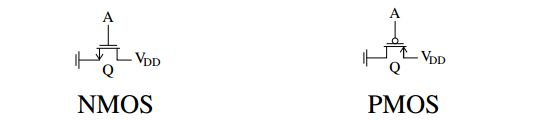
\includegraphics[scale=0.5]{nmos_and_pmos.jpg}
\end{center}
\caption{A PMOS transistor will be denoted with a little bubble to distinguish it from NMOS (diagram courtesy from Prof. Mann's lecture slides)}
\end{figure}
We'll combine both of these transistors to create a CMOS transistor.
\section{How gates compute Boolean values}
Depending on what current state each input is in (either 1 or 0) each respective transistor will either have a high or low resistance. A high resistance restricts any flow, whereas a low resistance allows for it. This means that based on the resistance of transistors in a given circuit, the flow will either have a clean path to power (denoted by 1) or ground (denoted by 0). \newpage
\begin{ex}
The filled in table from a CMOS diagram from Prof. Mann's slides on slide 2-16:
\end{ex}
\begin{center}
\begin{tabular}{ c c | c c c c | c}
$A$ & $B$ & $Q_1$ &$Q_2$ &$Q_3$ &$Q_4$ & $Z$ \\ \hline
0&0&LOW&LOW&HIGH&HIGH&1\\
0&1&LOW&HIGH&HIGH&LOW&1\\
1&0&HIGH&LOW&LOW&HIGH&1\\
1&1&HIGH&HIGH&LOW&LOW&0\\
\end{tabular}
\end{center}
\begin{figure}[ht]
\begin{center}
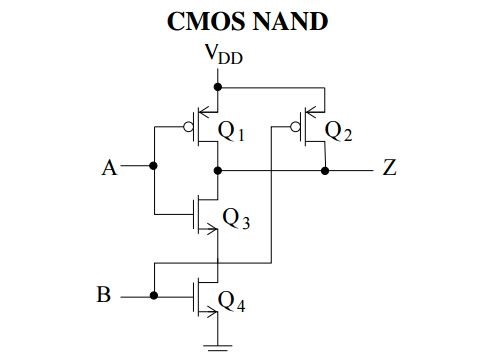
\includegraphics[scale=0.5]{nmos_diagram.jpg}
\end{center}
\caption{Inputs $A$ and $B$ are connected to their respective transistors. The flow from $Z$ can either flow towards power (1) or ground (0) (diagram courtesy from Prof. Mann's lecture slides)}
\end{figure}
\subsection{Deriving a Truth Table from a Circuit}
Interpreting a circuit is pretty simple:
\begin{itemize}
\item[1.] Find a gate whose all of its inputs are known
\item[2.] Compute its output
\item[3.] Repeat
\end{itemize}
\begin{ex}
Fill in the truth table defining this circuit diagram (diagram courtesy from Prof. Mann's lecture slides)
\end{ex}
\begin{figure}[ht]
\begin{center}
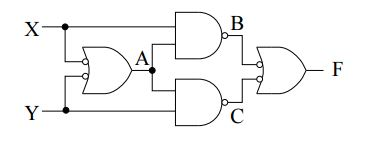
\includegraphics[scale=0.5]{circuit_diagram.jpg}
\end{center}
\end{figure}
Filling in the table yields
\begin{center}
\begin{tabular}{ c c | c c c | c}
$X$ & $Y$ & $A$ &$B$ &$C$ & $F$ \\ \hline
0 & 0 & 1 & 1 & 1 & 0\\
0 & 1 & 1 & 1 & 0 & 1\\
1 & 0 & 1 & 0 & 1 & 1\\
1 & 1 & 0 & 1 & 1 & 0\\
\end{tabular}
\end{center}
This is an XOR gate ($A \oplus B$), which returns 1 if one and only one input is true.
\subsubsection{To finish off...}
\subsection{Decoders}
This is a useful hardware component. A decoder converts binary to ``unary". With $n$ inputs, we'll have $2^n$ outputs. Because we designed the hardware, it is guaranteed that one of the $2^n$ outputs is 1.
%TODO include diagram I drew and table%

\subsection{Multiplexors (or Multiplexers)}
Based on inputs $S_0$ and $S_1$, a multiplexor determines which input $D_S$ to process (i.e., + - / *). For instance, if we want to add two values, we set $S_0$ and $S_1$ to certain values, and then we select the given output $D_S$ that outputs addition. More on this in the next lecture.
%END%
\end{document}